\documentclass[12pt,hyperref,a4paper,UTF8]{ctexart}
\usepackage{HDUReport}
\usepackage{listings}
\usepackage{xcolor}
\usepackage{graphicx}
\usepackage{setspace}
\usepackage{float}
\setstretch{1.5} % 设置全局行距为1.5倍

\usepackage{enumitem} % 载入enumitem包以便自定义列表环境
\setlist[itemize]{itemsep=0pt, parsep=0pt} % 设置itemize环境的项目间距和段落间距

\setmainfont{Times New Roman} % 英文正文为Times New Roman


\usepackage{tikz}
\usetikzlibrary{shapes.geometric, arrows}
\usetikzlibrary{positioning, arrows.meta}
\usetikzlibrary{calc}
%封面页设置
{   
    %标题
    \title{ 
        \vspace{1cm}
        \heiti \Huge \textbf{《单片机原理及应用》作业报告} \par
        \vspace{1cm} 
        \heiti \Large {\underline{大作业:串口屏秒表实物系统}   } 
        \vspace{3cm}
    
    }

    \author{
        \vspace{0.5cm}
        \kaishu\Large 学院\ \dlmu[9cm]{卓越学院} \\ %学院
        \vspace{0.5cm}
        \kaishu\Large 学号\ \dlmu[9cm]{23040409} \\ %班级
        \vspace{0.5cm}
        \kaishu\Large 姓名\ \dlmu[9cm]{付子豪} \qquad  \\ %学号
        \vspace{0.5cm}
        \kaishu\Large 专业\ \dlmu[9cm]{集成电路EDA} \qquad \\ %姓名 
    }
        
    \date{\today} % 默认为今天的日期,可以注释掉不显示日期
}
%%------------------------document环境开始------------------------%%
\begin{document}

%%-----------------------封面--------------------%%
\cover
\thispagestyle{empty} % 首页不显示页码
%%------------------摘要-------------%%
%\newpage
%\begin{abstract}




%\end{abstract}

%\thispagestyle{empty} % 首页不显示页码

%%--------------------------目录页------------------------%%
% \newpage
% \tableofcontents
% \thispagestyle{empty} % 目录不显示页码

%%------------------------正文页从这里开始-------------------%
\newpage
\setcounter{page}{1} % 让页码从正文开始编号

\section{系统功能概述}

\textbf{本系统实现实物51单片机数码管秒表功能,并通过TJC串口屏与51单片机的UART通信,并对其进行功能设置与控制}。秒表主要包含以下三大功能:

\begin{itemize}
  \item \textbf{计时器功能}:支持开始/暂停计时及复位操作,时间精度为0.01秒,最大计时范围为99分59秒99。通过串口屏或按键K1实现暂停/继续计时,按键K2实现复位功能,直观显示当前计时状态。
  
  \item \textbf{倒计时功能}:支持自定义设置倒计时时间(1秒至59分59秒),默认设置为1分钟。提供继续/暂停、复位操作,并在倒计时结束时通过三个LED指示灯同时亮起1秒进行提示。支持通过串口屏直接输入秒数进行精确设置。
  
  \item \textbf{E2PROM掉电存储功能}:利用AT24C02芯片实现数据掉电存储。无论在计时器还是倒计时模式下,均可将当前显示时间保存至AT24C02,并在需要时读取。这可用于记录重要时间点或恢复上次使用状态。
\end{itemize}

系统采用多模式设计,用户可以通过串口屏在计时器和倒计时模式之间自由切换。串口屏通信成功后,均有LED指示灯反馈,确保用户能够清晰了解当前系统态。数码管显示格式为"MM-SS-ss"(分钟--:百分秒),为用户提供精确的时间信息。

\begin{figure}[H] % [H] 表示强制当前位置插入
        \centering
        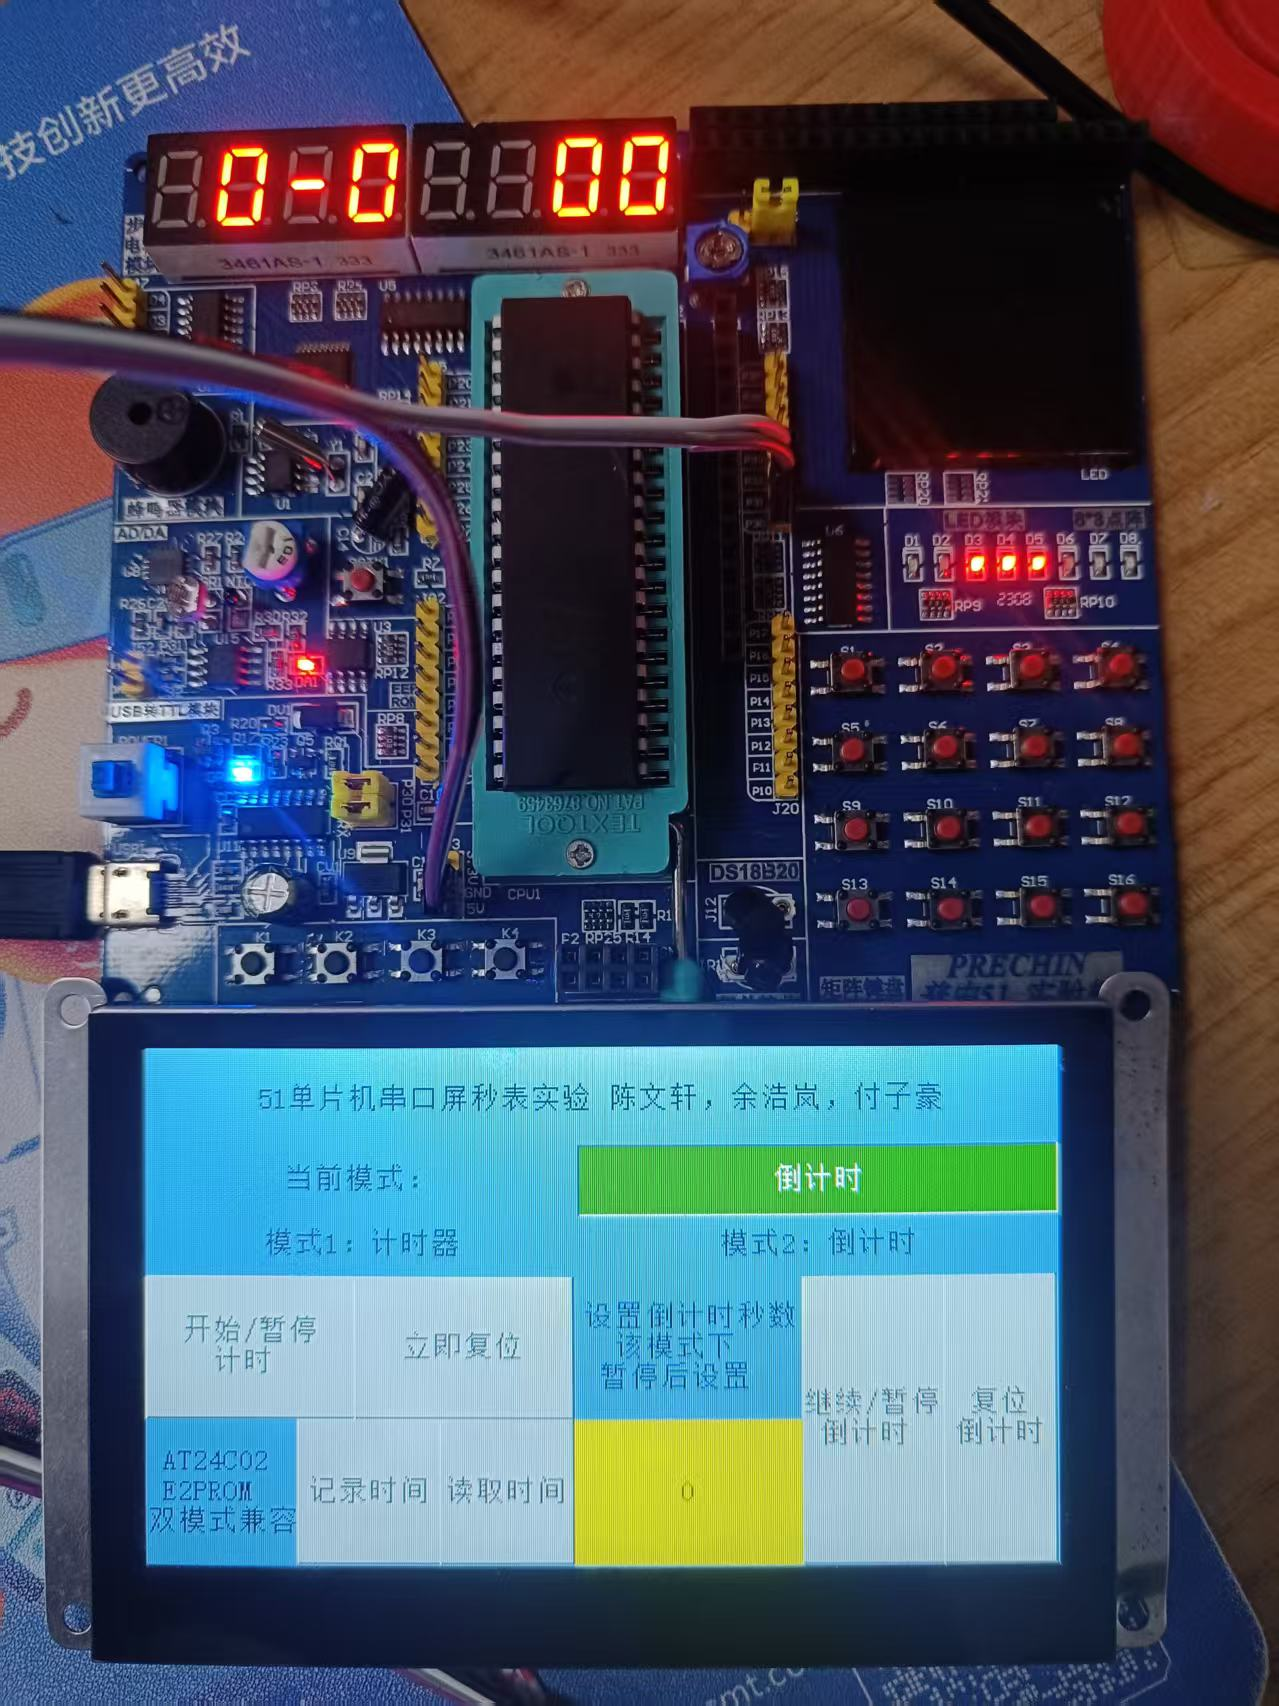
\includegraphics[width=0.50\textwidth]{figures/1.jpg} % 调整宽度为文本宽度的 80%
        \caption{系统实物图(相机刷新率问题,数码管拍照不全,肉眼观看不会有此问题)} %图片标题
        \label{fig:example} % 图片标签,用于引用
\end{figure}

\section{系统设计}

\subsection{硬件架构}

本系统的硬件架构由以下主要组件构成:

\begin{itemize}
  \item \textbf{控制核心}:51单片机(STC89C52RC),负责系统的核心控制逻辑,作为数码管驱动的主控制器
  \item \textbf{人机交互界面}:TJC串口屏,提供直观的操作界面,是系统的总输入集成
  \item \textbf{时间显示}:8位数码管,用于显示时间信息(分:秒:百分秒),是系统的主要输出
  \item \textbf{状态指示}:多个LED指示灯,包括UART命令响应指示灯和倒计时结束指示灯,可以直观的监控系统状态
  \item \textbf{数据存储}:AT24C02 EEPROM芯片,用于掉电数据存储,用于存贮时间
\end{itemize}

系统硬件构成总框图如下:

\begin{figure}[H]
    \centering
    % 这里可以插入系统连接示意图
    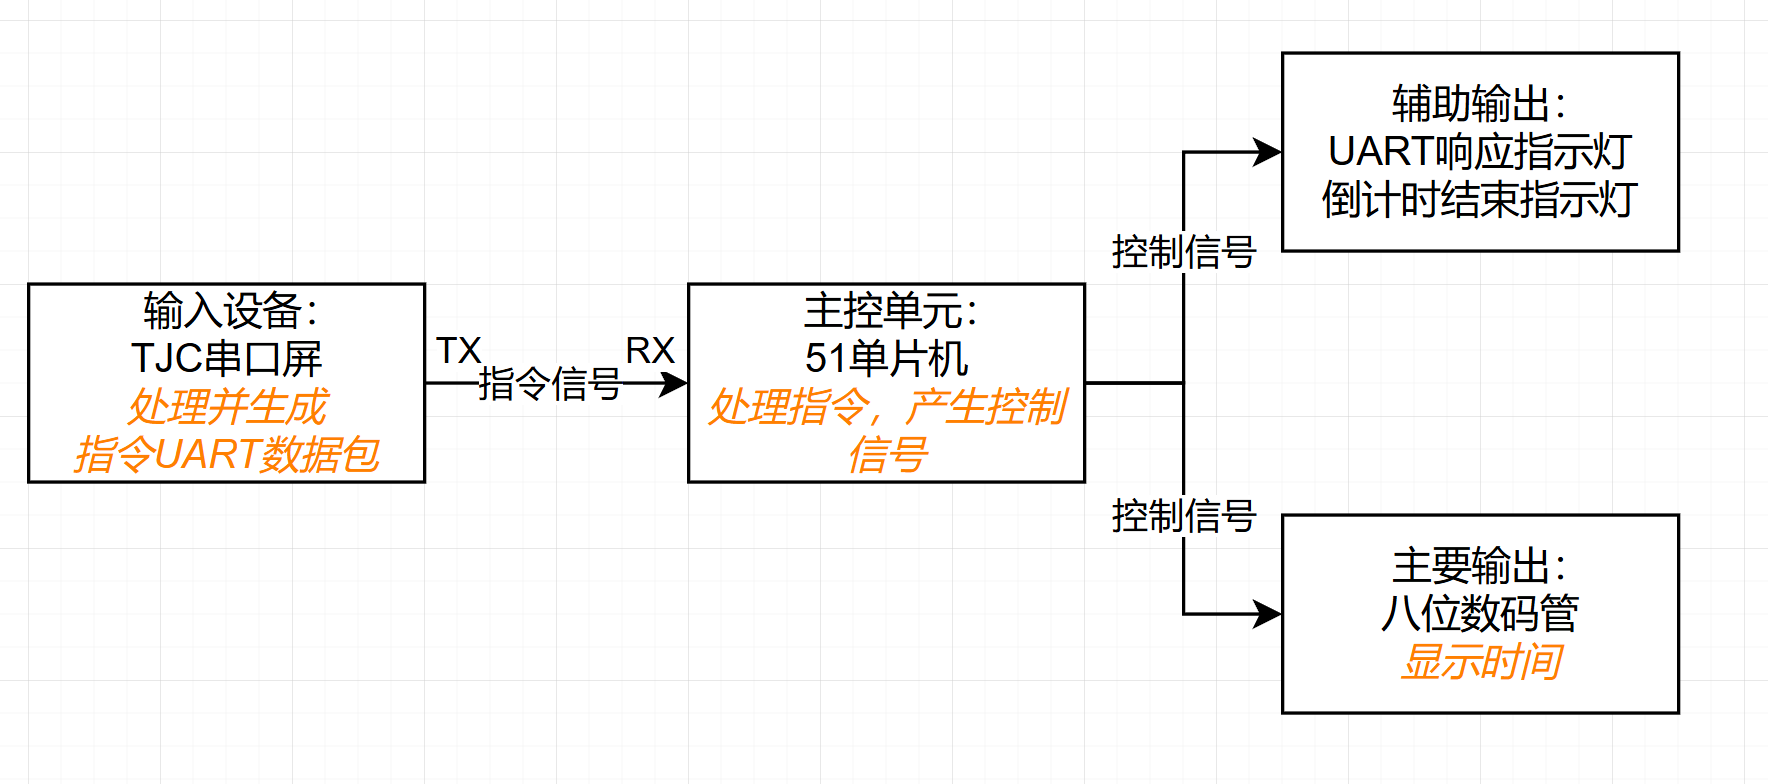
\includegraphics[width=0.9\textwidth]{figures/2.png} % 调整宽度为文本宽度的 80%
    \caption{系统功能总框图}
    \label{fig:hardware-connection}
\end{figure}

\subsection{软件架构}

软件设计采用模块化结构,包含以下主要模块:

\begin{itemize}
  \item \textbf{主控模块}:负责系统初始化和主循环控制,主要就是对八位数码管的显示逻辑进行针对UART指令的实时调整
  \item \textbf{定时器模块}:提供精确的时基,驱动数码管显示和按键扫描
  \item \textbf{UART通信模块}:处理串口屏与单片机间的数据交换
  \item \textbf{模式控制模块}:管理计时器和倒计时两种工作模式
  \item \textbf{数据存储模块}:实现AT24C02的读写操作
  \item \textbf{时间显示驱动模块}:控制数码管和LED的显示状态,并根据时分秒变量更新显示
\end{itemize}

同时,软件架构采用基于中断的工作方式,主要包括定时器中断和串口接收中断,确保系统实时响应外部输入并准确计时。

\begin{figure}[H]
    \centering
    % 这里可以插入系统连接示意图
    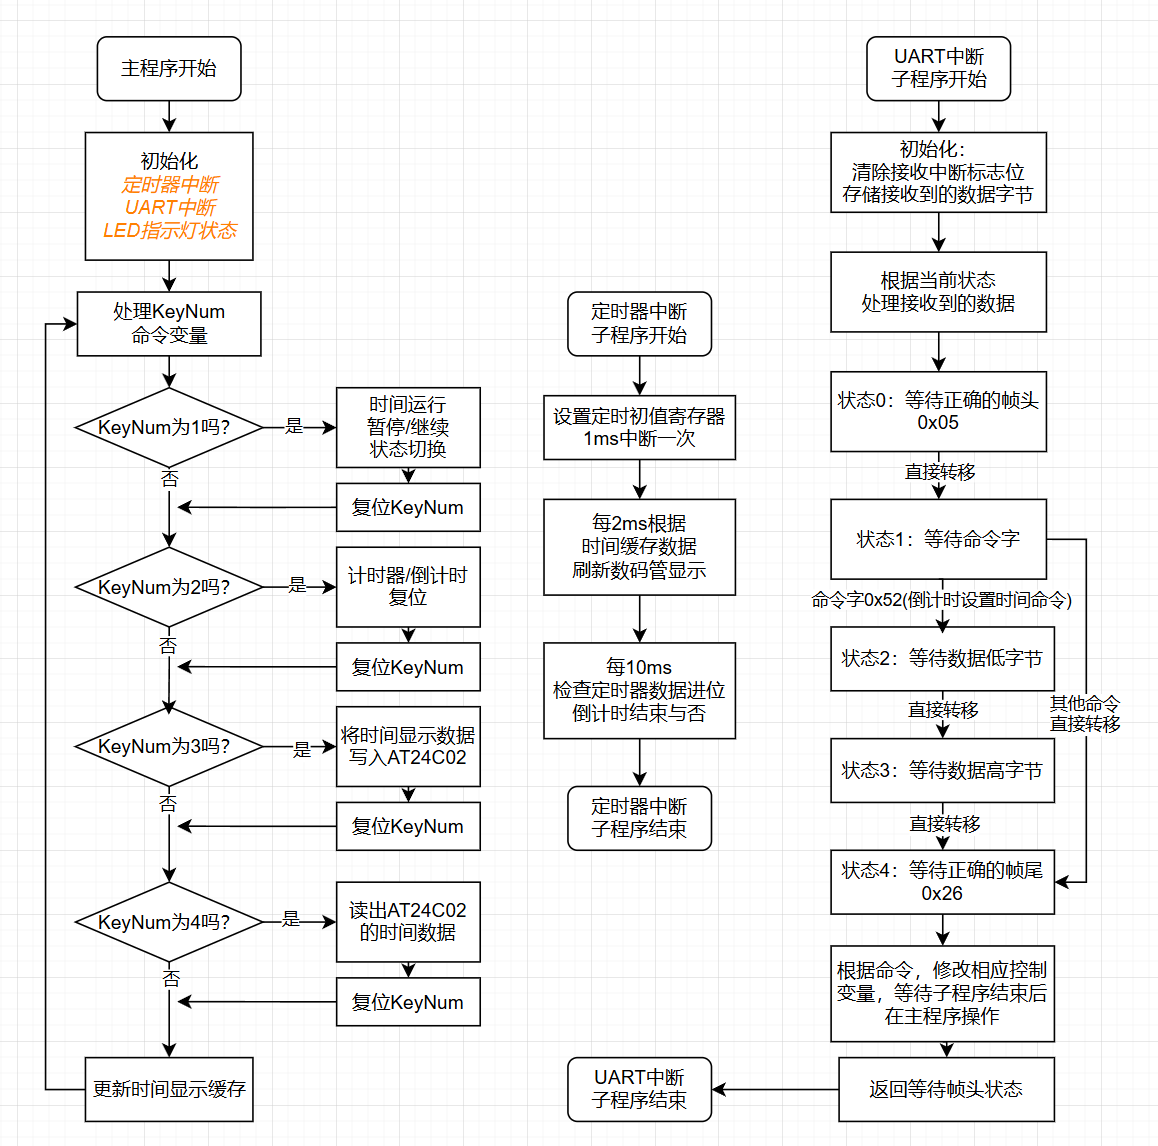
\includegraphics[width=0.9\textwidth]{figures/3.png} % 调整宽度为文本宽度的 80%
    \caption{主程序控制流程图}
    \label{fig:hardware-connection}
\end{figure}

\section{软件系统设计}

\subsection{简易UART协议}

本系统设计了一套简单有效的通信协议,用于串口屏与单片机之间的数据交换:

\subsubsection{协议格式}

每个通信帧由以下部分组成:
\begin{itemize}
  \item \textbf{帧头}:固定值0x05,标识数据帧开始
  \item \textbf{命令字}:表示操作类型,如0x30,就表示在计时器模式下的开始/暂停命令
  \item \textbf{数据字段}:只有0x52命令字下有效(倒计时设置命令),两个字节表示一个0-65535的秒数,小端模式表示数据
  \item \textbf{帧尾}:固定值0x26,标识数据帧结束
\end{itemize}

\subsubsection{命令集}

系统支持以下命令类型:

\begin{itemize}
  \item \textbf{计时器控制命令}
    \begin{itemize}
      \item 0x30:暂停/继续计时
      \item 0x31:复位计时器
      \item 0x32:将当前时间写入AT24C02
      \item 0x33:从AT24C02读取时间
    \end{itemize}
  
  \item \textbf{模式切换命令}
    \begin{itemize}
      \item 0x40:切换到计时器模式
      \item 0x41:切换到倒计时模式
    \end{itemize}
    
  \item \textbf{倒计时控制命令}
    \begin{itemize}
      \item 0x50:倒计时暂停/继续
      \item 0x51:倒计时复位
      \item 0x52:设置倒计时时间,后跟两字节表示秒数(低字节在前)
    \end{itemize}
\end{itemize}

通过该协议,串口屏可以完全控制51单片机秒表系统的各项功能,并实现人机交互界面的快速响应。

\subsection{数码管显示实现}

本系统采用8位动态扫描数码管作为主要时间显示设备,能够实时显示“分-秒-百分秒”格式的计时信息。显示实现主要包括以下几个方面:

\begin{itemize}
  \item \textbf{显示缓存区}:通过Nixie\_Buf数组作为显示缓冲区,主程序每次更新时间后,调用Nixie\_SetBuf函数将各位数字(如分钟、秒、百分秒)及分隔符“-”写入对应位置。
  \item \textbf{段码表}:NixieTable数组存储了0-9数字和“-”等符号的段码,便于快速查表显示。
  \item \textbf{动态扫描}:在定时器中断中周期性调用Nixie\_Loop函数,依次点亮每一位数码管,实现动态显示,避免鬼影和亮度不均。
  \item \textbf{位选与段选}:通过P2.2~P2.4控制位选,P0输出段码,实现对8位数码管的独立控制。
\end{itemize}

主循环根据当前计时状态实时刷新显示缓冲区,数码管显示内容始终与内部时间变量保持同步,保证显示的准确性和实时性。该模块结构清晰,便于维护和扩展。

\subsection{AT24C02 E2PROM掉电存储实现}

为实现掉电数据保存,系统采用AT24C02串行EEPROM芯片,通过I2C总线与单片机通信。主要实现方式如下:

\begin{itemize}
  \item \textbf{数据结构}:将当前分钟、秒、百分秒分别存储在AT24C02的0、1、2地址单元。
  \item \textbf{写入操作}:调用AT24C02\_WriteByte函数,依次将Min、Sec、MiniSec写入对应地址,写入后适当延时以确保数据可靠保存。
  \item \textbf{读取操作}:调用AT24C02\_ReadByte函数,从0、1、2地址读取数据,恢复到Min、Sec、MiniSec变量,实现断电后时间的恢复。
  \item \textbf{I2C协议}:底层通过I2C协议实现数据传输,包含起始、发送地址、数据、应答和停止等标准流程,保证通信的稳定性。
\end{itemize}

该功能支持用户通过按键或串口屏命令随时保存和恢复当前时间,极大提升了系统的实用性和可靠性,适用于需要断电记忆的应用场景。

\subsection{TJC串口屏设计}

串口屏不是51单片机的软件设计内容,在本实验中作为可编程外设与输入设备参与系统搭建,这里进行简要介绍。

\begin{figure}[H]
    \centering
    % 这里可以插入系统连接示意图
    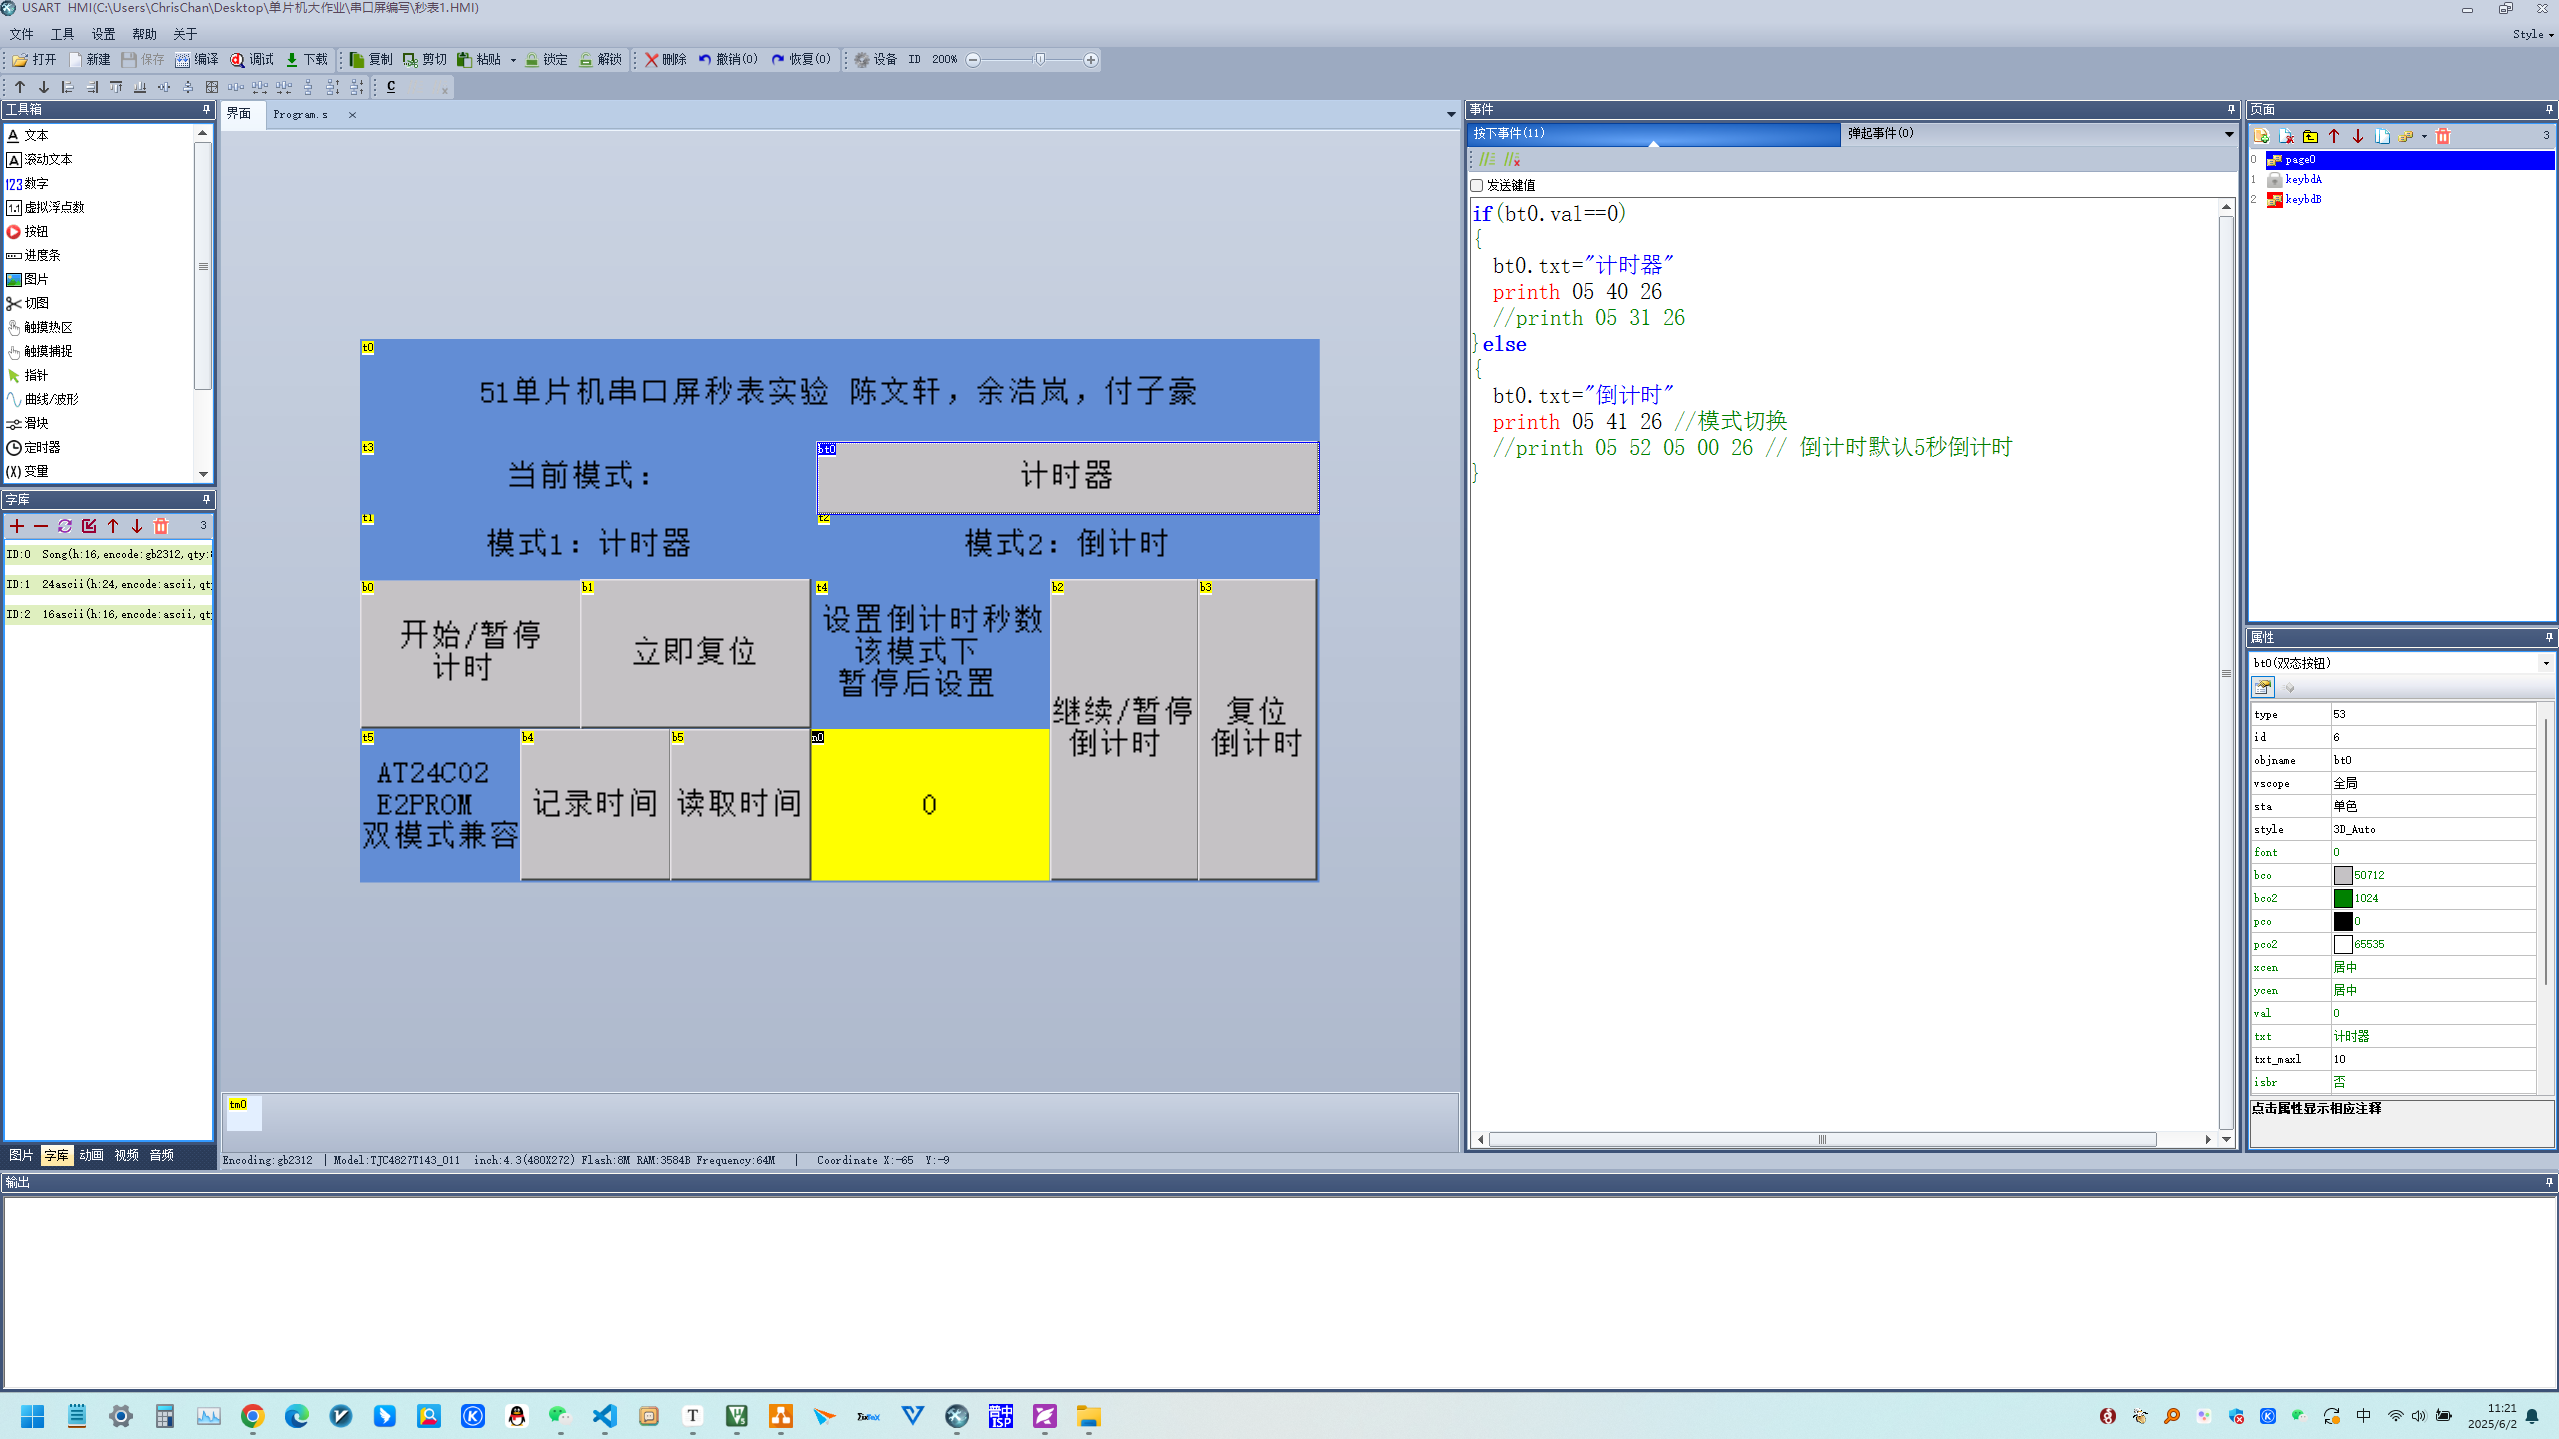
\includegraphics[width=0.9\textwidth]{figures/4.png} % 调整宽度为文本宽度的 80%
    \caption{TJC串口屏设计界面}
    \label{fig:hardware-connection}
\end{figure}

如图,串口屏设计主要包含两大部分。首先就是界面中虚拟按钮/文本框/整形数字框等模块的位置设定,需要进行位置对齐等美观化调整;
其次,对于主要输入的虚拟按钮,需要设计相应的按钮按下后,发送相应的UART数据命令包。如图中示例的是按下状态切换按钮后,根据当前
按钮状态,发送不同的状态数据包,并对模式按钮上的文字进行更改,以指示当前系统工作模式(计时器/倒计时)。其余按钮也按类似的逻辑进行设计。

其中,对于倒计时时间设置,串口屏导入了数字键盘界面,通过添加相应的控制逻辑(按下键盘“OK”键逻辑添加),即可发送键盘上的数值,自动生成相应的数据包,
最后传输给51单片机进行处理。

\begin{figure}[H]
    \centering
    % 这里可以插入系统连接示意图
    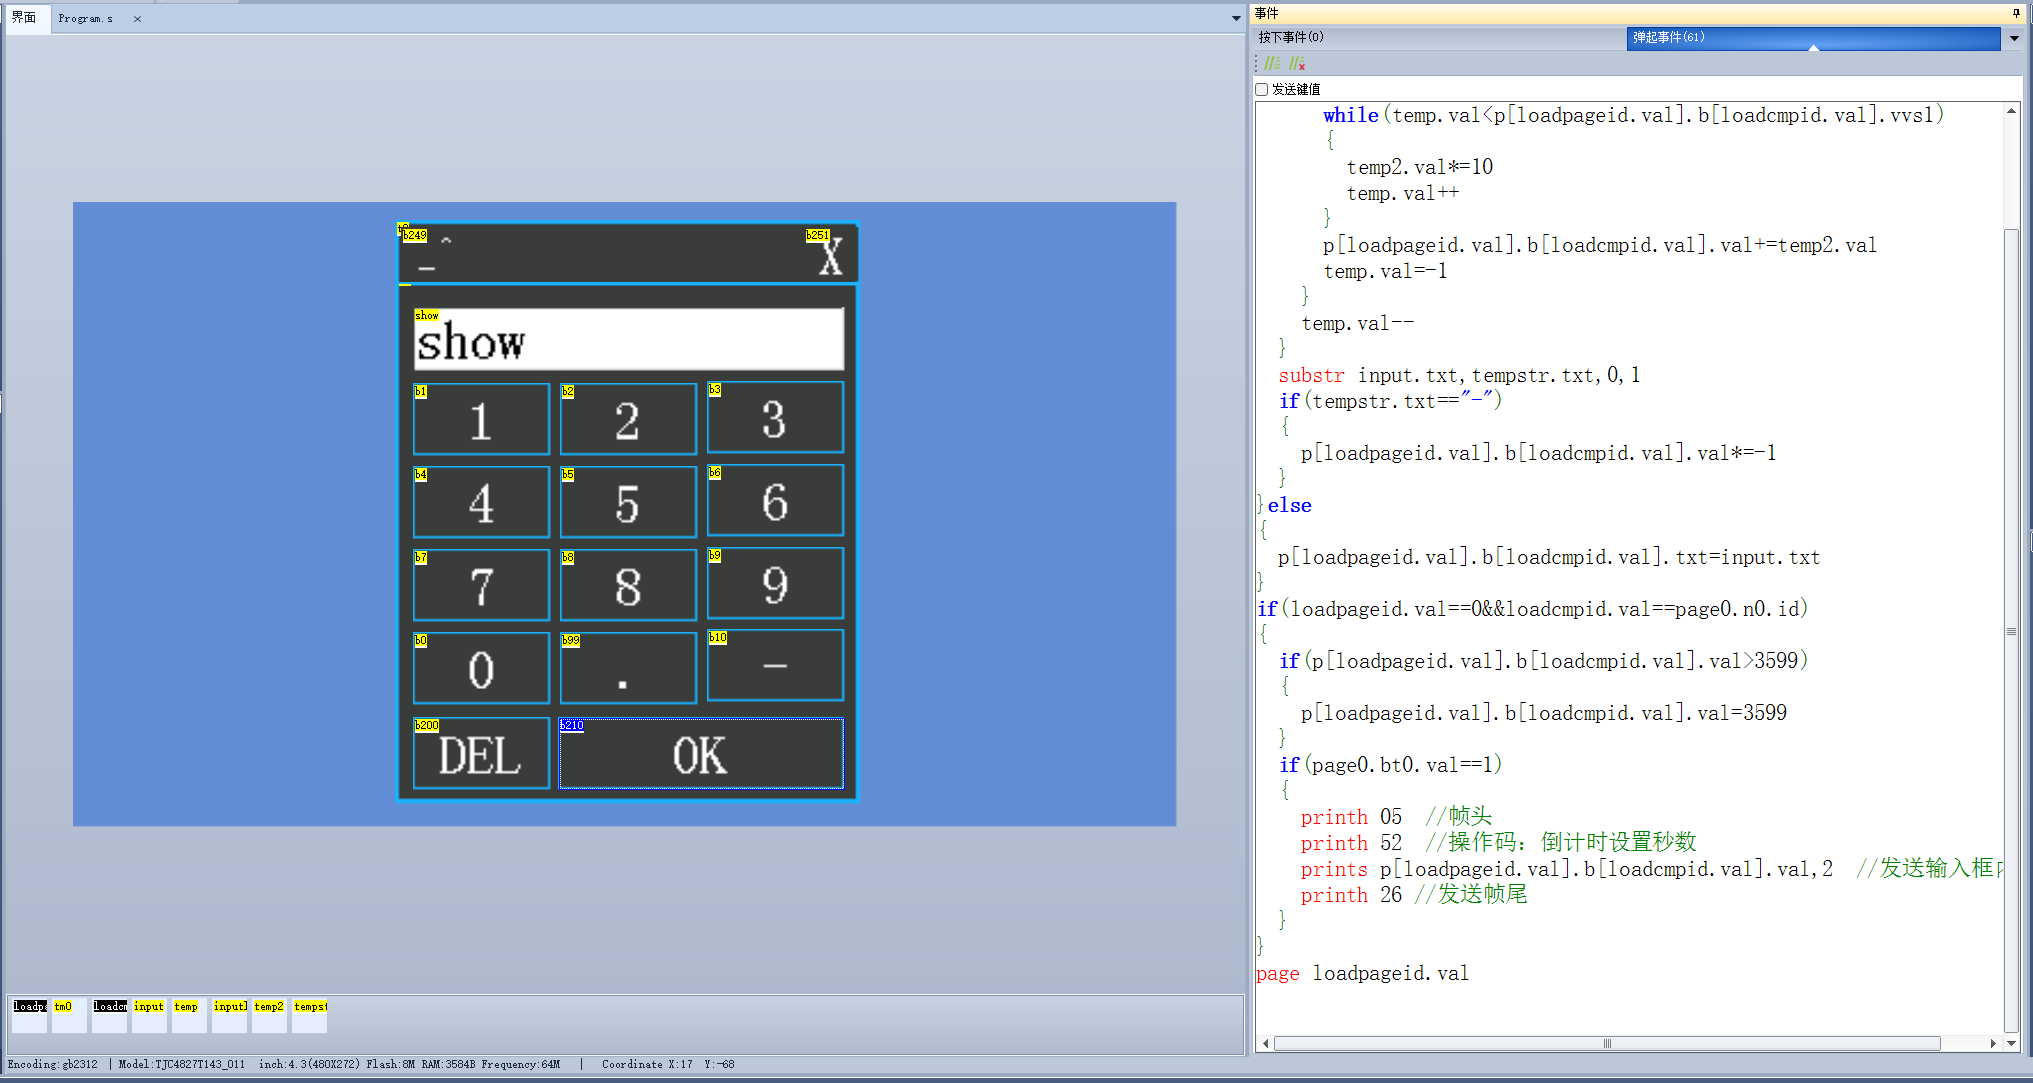
\includegraphics[width=0.9\textwidth]{figures/5.png} % 调整宽度为文本宽度的 80%
    \caption{串口屏数字键盘设计,右侧TJC代码就是数据发送逻辑}
    \label{fig:hardware-connection}
\end{figure}


\section{系统测试与结果}

本系统完成后进行了功能测试,测试结果表明系统能够稳定运行并满足设计要求:

\begin{itemize}
  \item 计时器功能:计时基本准确,暂停/继续和复位功能工作正常
  \item 倒计时功能:能够准确设置倒计时时间,倒计时结束LED提示正常
  \item 数据存储功能:能够正确保存和读取AT24C02中的时间数据
  \item 串口通信:稳定可靠,可实现所有功能的远程控制
\end{itemize}

\section{结论与展望}

本设计成功实现了基于51单片机的多功能秒表系统,通过串口屏实现了良好的人机交互。系统整体性能稳定,功能齐全,达到了预期的设计目标。

未来可考虑以下改进方向:
\begin{itemize}
  \item 增加更多计时模式,如lap计时、多段计时等
  \item 增强串口屏UI设计,提供更直观的用户界面
  \item 扩展存储功能,支持存储多组时间记录
  \item 添加蜂鸣器等声音提示功能,增强人机交互体验
\end{itemize}

\section{本成员分工}

本次大作业中,本人主要负责以下内容:

\begin{itemize}
  \item \textbf{EEPROM的I2C通信编写与调试}:独立完成了AT24C02 EEPROM的I2C底层驱动程序设计,包括I2C协议的实现、数据读写函数的开发与调试,确保掉电存储功能稳定可靠。针对实际硬件环境进行了多轮测试与优化,保证了数据在掉电情况下的正确保存与恢复。
  \item \textbf{最终报告的\LaTeX{}文档编写}:负责本次大作业最终报告的\LaTeX{}排版与内容整理,包括结构设计、图表插入、代码高亮、格式美化等。确保文档内容条理清晰、排版规范、便于后续查阅和展示。
\end{itemize}

在完成上述工作后,积极参与了系统整体联调与功能测试,协助团队成员解决软硬件集成过程中遇到的问题,推动了项目的顺利完成。
\section*{附录}


\begin{lstlisting}[language=C, caption={main.c 核心功能实现代码}]

#include <REGX52.H>
#include "Timer0.h"
#include "Key.h"
#include "Nixie.h"
#include "Delay.h"
#include "AT24C02.h"

unsigned char KeyNum;
unsigned char Min,Sec,MiniSec;
unsigned char RunFlag;

// 模式控制变量
#define MODE_TIMER 0       // 计时器模式
#define MODE_COUNTDOWN 1   // 倒计时模式
unsigned char CurrentMode = MODE_TIMER;  // 默认为计时器模式

// 倒计时设置值
unsigned char CDMin = 1, CDSec = 0, CDMiniSec = 0; // 倒计时默认值:1分钟

// LED灯的定义
#define LED P2_0
#define CD_LED1 P2_5      // 倒计时结束指示灯1
#define CD_LED2 P2_6      // 倒计时结束指示灯2
#define CD_LED3 P2_7      // 倒计时结束指示灯3
unsigned char led_state = 1;    
unsigned char DEAL_LED = 0; //正确处理指令后,再闪灯
// 定义通信协议
#define FRAME_HEADER 0x05  // 帧头
#define FRAME_FOOTER 0x26  // 帧尾

//计时器指令
#define CMD_STOP_OR_CONTINUE 0x30 // 命令:暂停/继续计时器 
#define CMD_RESET 0x31 //命令:RESET计时器
#define CMD_WRITE_AT 0x32 //命令:将当前时间放入AT存储器
#define CMD_READ_AT 0x33 //命令:读取AT存储器,覆盖当前时间

// 模式切换指令
#define CMD_MODE_TIMER 0x40      // 切换到计时器模式
#define CMD_MODE_COUNTDOWN 0x41  // 切换到倒计时模式

// 倒计时控制指令
#define CMD_CD_PAUSE_CONTINUE 0x50  // 倒计时暂停/继续
#define CMD_CD_RESET 0x51          // 倒计时复位到设定值
#define CMD_CD_SET_TIME 0x52       // 设置倒计时时间

// 通信协议变量
unsigned char rx_state = 0;     // 接收状态:0-等待帧头,1-等待操作数,2-等待数据低字节,3-等待数据高字节,4-等待帧尾
unsigned char rx_command = 0;   // 接收到的操作数
unsigned int rx_time_data = 0;  // 接收到的时间数据(秒数)
unsigned char rx_time_low = 0;  // 接收到的时间数据低字节
unsigned char rx_time_high = 0; // 接收到的时间数据高字节

void uart_init(unsigned int baud) //9600:0XFA
{
	TMOD |= 0X20; // 设置计数器工作方式2
	SCON = 0X50; // 设置为工作方式1
	PCON = 0X80; // 波特率加倍
	TH1 = baud; // 计数器初始值设置
	TL1 = baud;

	// 配置中断器
	ES = 1; // 打开接收中断
	EA = 1; // 打开总中断
	TR1 =1 ; // 打开计数器		
}

// 将所有倒计时指示LED设置为指定状态
void SetCountdownLEDs(bit state)
{
    CD_LED1 = state;
    CD_LED2 = state;
    CD_LED3 = state;
}

void main()
{
	Timer0_Init();
	uart_init(0XFA); // 波特率为9600
	// 初始化LED状态
	LED = 0;  // 初始状态为点亮(低电平)
	led_state = 0;
	
	// 初始化倒计时LED为熄灭状态
	SetCountdownLEDs(1);  // 高电平熄灭
	
	while(1)
	{
		// 处理按键和命令
		if(KeyNum==1)     // K1按键按下
		{
			if(CurrentMode == MODE_TIMER)
			{
				RunFlag=!RunFlag;    // 计时器模式:启动标志位翻转
			}
			else // 倒计时模式
			{
				RunFlag=!RunFlag;    // 倒计时模式也使用相同的运行标志
			}
			KeyNum = 0; //处理完成,状态复位
			DEAL_LED=1;
		}
		if(KeyNum==2)     // K2按键按下
		{
			if(CurrentMode == MODE_TIMER)
			{
				Min=0;              // 计时器模式:分秒清0
				Sec=0;
				MiniSec=0;
			}
			else // 倒计时模式
			{
				Min=CDMin;          // 倒计时模式:复位到设定值
				Sec=CDSec;
				MiniSec=CDMiniSec;
				SetCountdownLEDs(1); // 复位指示灯
			}
			KeyNum = 0; //处理完成,状态复位

		}
		if(KeyNum==3)			//K3按键按下
		{
			AT24C02_WriteByte(0,Min);	//将分秒写入AT24C02
			Delay(5);
			AT24C02_WriteByte(1,Sec);
			Delay(5);
			AT24C02_WriteByte(2,MiniSec);
			Delay(5);
			KeyNum = 0; //处理完成,状态复位

		}
		if(KeyNum==4)			//K4按键按下
		{
			Min=AT24C02_ReadByte(0);	//读出AT24C02数据
			Sec=AT24C02_ReadByte(1);
			MiniSec=AT24C02_ReadByte(2);
			KeyNum = 0; //处理完成,状态复位

		}
		// 显示当前时间
		Nixie_SetBuf(1,Min/10);    //设置显示缓存,显示数据
		Nixie_SetBuf(2,Min%10);
		Nixie_SetBuf(3,11);
		Nixie_SetBuf(4,Sec/10);
		Nixie_SetBuf(5,Sec%10);
		Nixie_SetBuf(6,11);
		Nixie_SetBuf(7,MiniSec/10);
		Nixie_SetBuf(8,MiniSec%10);
	}
}

/**
  * @brief  时间驱动函数,在中断中调用,根据当前模式执行不同操作
  * @param  无
  * @retval 无
  */
void Sec_Loop(void)
{
	if(RunFlag)
	{
		if(CurrentMode == MODE_TIMER) // 计时器模式
		{
			MiniSec++;
			if(MiniSec>=100)
			{
				MiniSec=0;
				Sec++;
				if(Sec>=60)
				{
					Sec=0;
					Min++;
					if(Min>=60)
					{
						Min=0;
					}
				}
			}
		}
		else // 倒计时模式
		{
			if(Min==0 && Sec==0 && MiniSec==0)
			{
				// 倒计时已经结束,停止运行
				RunFlag = 0;
				
				// 点亮指示灯
				SetCountdownLEDs(0);  // 低电平点亮
				Delay(1000);         // 延时1秒
				SetCountdownLEDs(1);  // 熄灭指示灯
				
				return;
			}
			
			// 倒计时逻辑
			if(MiniSec==0)
			{
				if(Sec==0)
				{
					if(Min!=0)
					{
						Min--;
						Sec=59;
						MiniSec=99;
					}
				}
				else
				{
					Sec--;
					MiniSec=99;
				}
			}
			else
			{
				MiniSec--;
			}
		}
	}
}

// 串口通信中断函数
void uart() interrupt 4
{
	unsigned char rec_data; // 接收到的数据
										  
	RI = 0;	// 清除接收中断标志位

	rec_data = SBUF; // 存储接收到的数据
	SBUF = rec_data; // 将接收到的数据放入到发送寄存器
	
	// 根据当前状态处理接收到的数据
	switch (rx_state) {
		case 0: // 等待帧头
			if (rec_data == FRAME_HEADER) {
				rx_state = 1; // 进入等待操作数状态
			}
			break;
			
		case 1: // 等待操作数
			rx_command = rec_data; // 保存操作数
			if (rx_command == CMD_CD_SET_TIME) { 
				rx_state = 2; // 如果是设置时间命令,进入等待数据低字节状态
			} else {
				rx_state = 4; // 否则直接进入等待帧尾状态
			}
			break;
			
		case 2: // 等待数据低字节
			rx_time_low = rec_data;  // 保存时间数据低字节
			rx_state = 3;  // 进入等待数据高字节状态
			break;
			
		case 3: // 等待数据高字节
			rx_time_high = rec_data;  // 保存时间数据高字节
			rx_state = 4;  // 进入等待帧尾状态
			break;
			
		case 4: // 等待帧尾
			if (rec_data == FRAME_FOOTER) 
			{
				// 完整接收到一帧数据,根据操作数执行相应操作
				
				// 计时器模式命令
				if (rx_command == CMD_STOP_OR_CONTINUE && CurrentMode == MODE_TIMER)
				{
					KeyNum = 1; //计时器暂停/继续
					DEAL_LED=1;
				}
				else if (rx_command == CMD_RESET && CurrentMode == MODE_TIMER)
				{
					KeyNum = 2; //计时器复位
					DEAL_LED=1;
				}
				else if (rx_command == CMD_WRITE_AT)
				{
					KeyNum = 3; //将当前时间写入AT24C02
					DEAL_LED=1;
				}
				else if (rx_command == CMD_READ_AT)
				{
					KeyNum = 4; //从AT24C02读取时间
					DEAL_LED=1;
				}
				// 模式切换命令
				else if (rx_command == CMD_MODE_TIMER)
				{
					CurrentMode = MODE_TIMER;
					RunFlag = 0;  // 切换模式时停止计时
					Min = 0;
					Sec = 0;
					MiniSec = 0;
					DEAL_LED=1;
				}
				else if (rx_command == CMD_MODE_COUNTDOWN)
				{
					CurrentMode = MODE_COUNTDOWN;
					RunFlag = 0;  // 切换模式时停止计时
					Min = CDMin;  // 设置为默认倒计时值
					Sec = CDSec;
					MiniSec = CDMiniSec;
					DEAL_LED=1;
				}
				// 倒计时控制命令
				else if (rx_command == CMD_CD_PAUSE_CONTINUE && CurrentMode == MODE_COUNTDOWN)
				{
					if (CurrentMode == MODE_COUNTDOWN)
					{
						KeyNum = 1; // 倒计时暂停/继续
					}
					DEAL_LED=1;
				}
				else if (rx_command == CMD_CD_RESET && CurrentMode == MODE_COUNTDOWN)
				{
					if (CurrentMode == MODE_COUNTDOWN)
					{
						KeyNum = 2; // 倒计时复位到设定值
					}
					DEAL_LED=1;
				}
				// 设置倒计时时间
				else if (rx_command == CMD_CD_SET_TIME && CurrentMode == MODE_COUNTDOWN) 
				{
	
					// 合并两个字节得到总秒数
					rx_time_data = (unsigned int)rx_time_high << 8 | rx_time_low;
					if (rx_time_data > 3599) // 最大支持59分59秒
					{
						rx_time_data = 3599; // 限制最大值为59分59秒
					}
					else if (rx_time_data <= 1) // 最小值为1秒
					{
						rx_time_data = 1; // 限制最小值为1秒
					}
					// 计算分和秒
					CDMin = rx_time_data / 60;
					CDSec = rx_time_data % 60;
					CDMiniSec = 0;
					
					// 如果当前是倒计时模式并且没有在运行,则立即更新显示
					if (CurrentMode == MODE_COUNTDOWN && RunFlag == 0)
					{
						Min = CDMin;
						Sec = CDSec;
						MiniSec = CDMiniSec;
					}
					DEAL_LED=1;
				}
				if (DEAL_LED) // 如果需要闪烁LED指示
				{
					// 执行LED闪烁 指示收到了UART数据包 并处理了
					LED = 0;  // 点亮LED (低电平点亮)
					Delay(50);  // 延时50ms
					LED = 1;  // 熄灭LED
				}

			}
			// 不管帧尾是否正确,都回到等待帧头状态
			rx_state = 0;
			break;
	}

	while(!TI);	// 等待发送数据完成
	TI = 0; // 清除发送完成标志位				
}

void Timer0_Routine() interrupt 1
{
	static unsigned int T0Count1,T0Count2,T0Count3;
	TL0 = 0x18;		//设置定时初值
	TH0 = 0xFC;		//设置定时初值
	T0Count1++;
	if(T0Count1>=20)
	{
		T0Count1=0;
		Key_Loop();	//20ms调用一次按键驱动函数
	}
	T0Count2++;
	if(T0Count2>=2)
	{
		T0Count2=0;
		Nixie_Loop();//2ms调用一次数码管驱动函数
	}
	T0Count3++;
	if(T0Count3>=10)
	{
		T0Count3=0;
		Sec_Loop();	//10ms调用一次数秒表驱动函数
	}
}

\end{lstlisting}

\begin{lstlisting}[language=C, caption={Nixie.c 数码管显示实现代码}]

#include <REGX52.H>
#include "Delay.h"

//数码管显示缓存区
unsigned char Nixie_Buf[9]={0,10,10,10,10,10,10,10,10};

//数码管段码表
unsigned char NixieTable[]={0x3F,0x06,0x5B,0x4F,0x66,0x6D,0x7D,0x07,0x7F,0x6F,0x00,0x40};

/**
  * @brief  设置显示缓存区
  * @param  Location 要设置的位置,范围:1~8
  * @param  Number 要设置的数字,范围:段码表索引范围
  * @retval 无
  */
void Nixie_SetBuf(unsigned char Location,Number)
{
	Nixie_Buf[Location]=Number;
}

/**
  * @brief  数码管扫描显示
  * @param  Location 要显示的位置,范围:1~8
  * @param  Number 要显示的数字,范围:段码表索引范围
  * @retval 无
  */
void Nixie_Scan(unsigned char Location,Number)
{
	P0=0x00;				//段码清0,消影
	switch(Location)		//位码输出
	{
		case 1:P2_4=1;P2_3=1;P2_2=1;break;
		case 2:P2_4=1;P2_3=1;P2_2=0;break;
		case 3:P2_4=1;P2_3=0;P2_2=1;break;
		case 4:P2_4=1;P2_3=0;P2_2=0;break;
		case 5:P2_4=0;P2_3=1;P2_2=1;break;
		case 6:P2_4=0;P2_3=1;P2_2=0;break;
		case 7:P2_4=0;P2_3=0;P2_2=1;break;
		case 8:P2_4=0;P2_3=0;P2_2=0;break;
	}
	P0=NixieTable[Number];	//段码输出
}

/**
  * @brief  数码管驱动函数,在中断中调用
  * @param  无
  * @retval 无
  */
void Nixie_Loop(void)
{
	static unsigned char i=1;
	Nixie_Scan(i,Nixie_Buf[i]);
	i++;
	if(i>=9){i=1;}
}


\end{lstlisting}


\begin{lstlisting}[language=C, caption={AT24C02.c E2PROM掉电存储实现代码}]

#include <REGX52.H>
#include "I2C.h"

#define AT24C02_ADDRESS		0xA0

/**
  * @brief  AT24C02写入一个字节
  * @param  WordAddress 要写入字节的地址
  * @param  Data 要写入的数据
  * @retval 无
  */
void AT24C02_WriteByte(unsigned char WordAddress,Data)
{
	I2C_Start();
	I2C_SendByte(AT24C02_ADDRESS);
	I2C_ReceiveAck();
	I2C_SendByte(WordAddress);
	I2C_ReceiveAck();
	I2C_SendByte(Data);
	I2C_ReceiveAck();
	I2C_Stop();
}

/**
  * @brief  AT24C02读取一个字节
  * @param  WordAddress 要读出字节的地址
  * @retval 读出的数据
  */
unsigned char AT24C02_ReadByte(unsigned char WordAddress)
{
	unsigned char Data;
	I2C_Start();
	I2C_SendByte(AT24C02_ADDRESS);
	I2C_ReceiveAck();
	I2C_SendByte(WordAddress);
	I2C_ReceiveAck();
	I2C_Start();
	I2C_SendByte(AT24C02_ADDRESS|0x01);
	I2C_ReceiveAck();
	Data=I2C_ReceiveByte();
	I2C_SendAck(1);
	I2C_Stop();
	return Data;
}

\end{lstlisting}
\begin{lstlisting}[language=C, caption={I2C.c I2C通信功能实现代码}]
#include <REGX52.H>

sbit I2C_SCL=P2^1;
sbit I2C_SDA=P2^0;

/**
  * @brief  I2C开始
  * @param  无
  * @retval 无
  */
void I2C_Start(void)
{
	I2C_SDA=1;
	I2C_SCL=1;
	I2C_SDA=0;
	I2C_SCL=0;
}

/**
  * @brief  I2C停止
  * @param  无
  * @retval 无
  */
void I2C_Stop(void)
{
	I2C_SDA=0;
	I2C_SCL=1;
	I2C_SDA=1;
}

/**
  * @brief  I2C发送一个字节
  * @param  Byte 要发送的字节
  * @retval 无
  */
void I2C_SendByte(unsigned char Byte)
{
	unsigned char i;
	for(i=0;i<8;i++)
	{
		I2C_SDA=Byte&(0x80>>i);
		I2C_SCL=1;
		I2C_SCL=0;
	}
}

/**
  * @brief  I2C接收一个字节
  * @param  无
  * @retval 接收到的一个字节数据
  */
unsigned char I2C_ReceiveByte(void)
{
	unsigned char i,Byte=0x00;
	I2C_SDA=1;
	for(i=0;i<8;i++)
	{
		I2C_SCL=1;
		if(I2C_SDA){Byte|=(0x80>>i);}
		I2C_SCL=0;
	}
	return Byte;
}

/**
  * @brief  I2C发送应答
  * @param  AckBit 应答位,0为应答,1为非应答
  * @retval 无
  */
void I2C_SendAck(unsigned char AckBit)
{
	I2C_SDA=AckBit;
	I2C_SCL=1;
	I2C_SCL=0;
}

/**
  * @brief  I2C接收应答位
  * @param  无
  * @retval 接收到的应答位,0为应答,1为非应答
  */
unsigned char I2C_ReceiveAck(void)
{
	unsigned char AckBit;
	I2C_SDA=1;
	I2C_SCL=1;
	AckBit=I2C_SDA;
	I2C_SCL=0;
	return AckBit;
}
 

\end{lstlisting}

%代码与图片模板,别删

% \begin{lstlisting}[language=C, caption={main.c 核心功能实现代码}]

% \end{lstlisting}

% \begin{figure}[H]
%     \centering
%     % 这里可以插入系统连接示意图
%     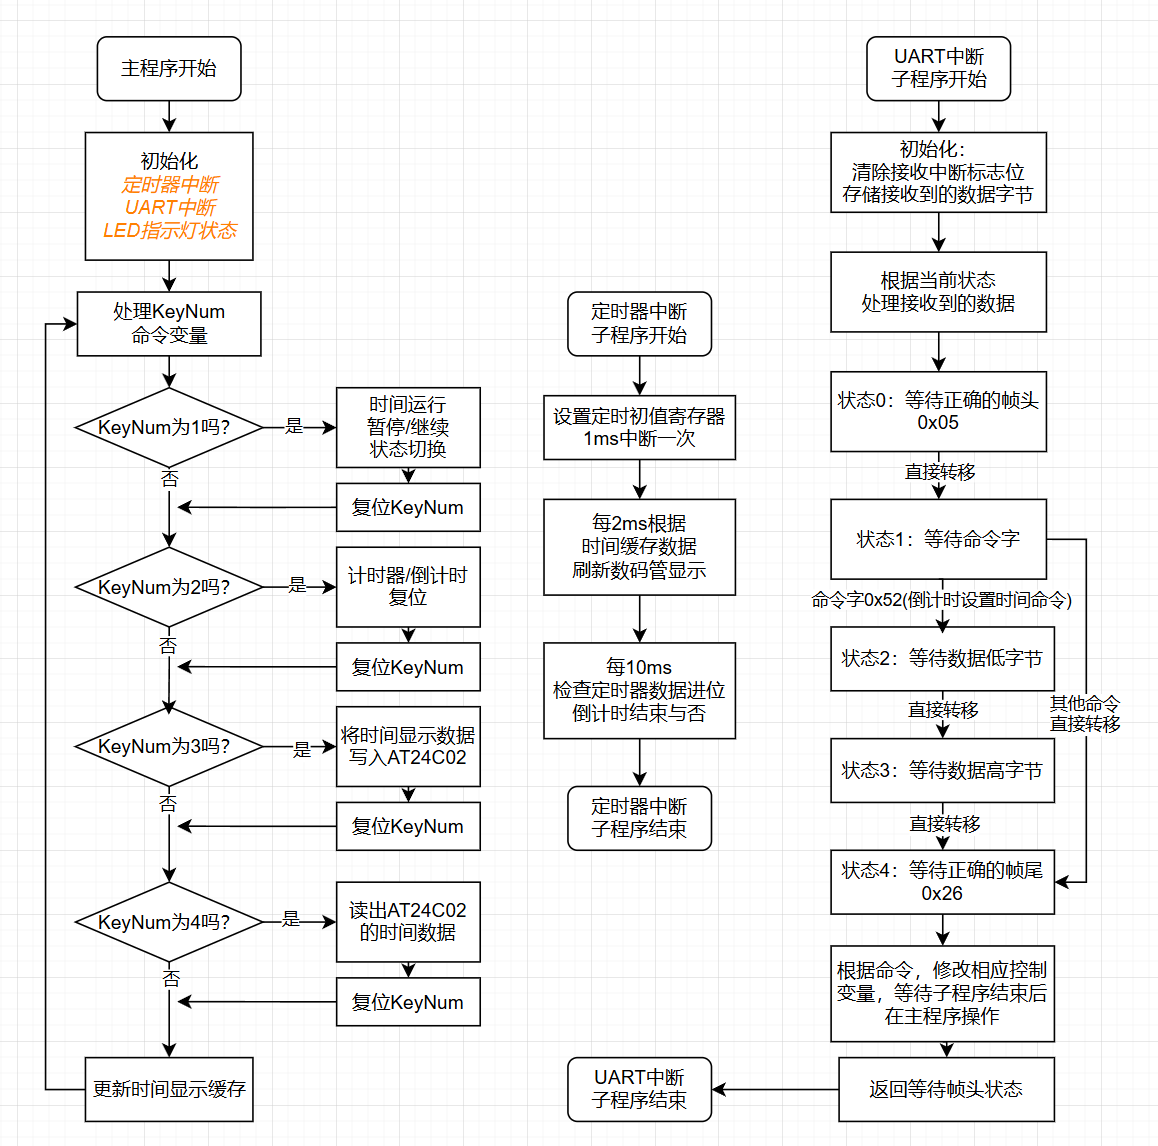
\includegraphics[width=0.9\textwidth]{figures/3.png} % 调整宽度为文本宽度的 80%
%     \caption{主程序控制流程图}
%     \label{fig:hardware-connection}
% \end{figure}

\end{document}